
\documentclass[12pt,hyperref={CJKbookmarks=true}]{beamer} %14pt为字体尺寸,默认值11pt.有8-12;14;17;20;bigger;smaller
\usepackage{ifthen}
%\usepackage[a3paper,landscape,showframe,margin=1.25in]{geometry}
%\usepackage[a3paper,landscape,margin=1.1in]{geometry}
\usepackage[a3paper,landscape,top=1.25in,bottom=0.8in,left=1in,right=1in]{geometry}
\usepackage{tikz,units}
\usepackage{circuitikz}
\usepackage{subfig}
\usetikzlibrary{backgrounds,circuits.ee.IEC.relay}
\usetikzlibrary{positioning}
\usepackage{tikzsymbols}
\usepackage{pgffor}
\usetikzlibrary {math}
\usepackage{lastpage}
\usepackage{fancyhdr}
\pagestyle{fancy}
\fancyhf{}
\fancyhead[ER,OL]{\heiti \zihao{-5} 热工专业图纸}
\fancyhead[OR,EL]{\heiti \zihao{-5} \leftmark}
\fancyfoot[CE,CO]{热工专业图纸~第~\thepage~页(共 \pageref{LastPage} 页)}
\renewcommand{\headrulewidth}{0.4pt}
\renewcommand{\footrulewidth}{0.4pt}
\tikzset{
box/.style={rectangle,minimum height=17pt,minimum width=20pt,text=red}
}
\tikzset{
boxA/.style={rectangle,minimum height=17pt,minimum width=20pt,draw=black}
}
\tikzset{
boxB/.style={rectangle,minimum height=17pt,minimum width=30pt,draw=black}
}
\tikzset{
boxC/.style={rectangle,minimum height=17pt,minimum width=120pt,draw=black}
}
\tikzset{
boxD/.style={minimum width=140pt,above left}
}
 % 載入封包與文檔配置
% 参考文献样式
% 使用biblatex-gb7714-2015宏包提供的\footfullcite命令实现脚注引用。
\usepackage[backend=biber,autolang=hyphen,style=gb7714-2015,
gbtype=true,gbalign=gb7714-2015,
doi=false,url=false,isbn=false]{biblatex}
\tikzset{
dpu/.style={rectangle,rounded corners=2pt,
minimum width=35pt,minimum height=40pt,inner sep=5pt,
draw=black,fill=black!20,scale=0.8},
switch/.style={rectangle,rounded corners=5pt,
minimum width=15pt,minimum height=50pt,inner sep=5pt,
draw=black,fill=black!20}
}




\makeatletter
\def\progressbar@progressbar{} % the progress bar
\newcount\progressbar@tmpcounta% auxiliary counter
\newcount\progressbar@tmpcountb% auxiliary counter
\newdimen\progressbar@pbht %progressbar height
\newdimen\progressbar@pbwd %progressbar width
\newdimen\progressbar@rcircle % radius for the circle
\newdimen\progressbar@tmpdim % auxiliary dimension

\progressbar@pbwd=\linewidth
\progressbar@pbht=1pt
\progressbar@rcircle=2.5pt

% the progress bar
\def\progressbar@progressbar{%

    \progressbar@tmpcounta=\insertframenumber
    \progressbar@tmpcountb=\inserttotalframenumber
    \progressbar@tmpdim=\progressbar@pbwd
    \multiply\progressbar@tmpdim by \progressbar@tmpcounta
    \divide\progressbar@tmpdim by \progressbar@tmpcountb

  \begin{tikzpicture}
    \draw[pbblue!30,line width=\progressbar@pbht]
      (0pt, 0pt) -- ++ (\progressbar@pbwd,0pt);

    \filldraw[pbblue!30] %
      (\the\dimexpr\progressbar@tmpdim-\progressbar@rcircle\relax, .5\progressbar@pbht) circle (\progressbar@rcircle);

    \node[draw=pbblue!30,text width=4em,align=center,inner sep=1pt,
      text=pbblue!70,anchor=east] at (0,0) {\textnormal{%
             \pgfmathparse{\insertframenumber*100/\inserttotalframenumber}%
             \pgfmathprintnumber[fixed,precision=2]{\pgfmathresult}\,\%%
        }%
};
  \end{tikzpicture}%
}

\addtobeamertemplate{headline}{}
{%
  \begin{beamercolorbox}[wd=\paperwidth,ht=4ex,center,dp=1ex]{white}%
    \progressbar@progressbar%
  \end{beamercolorbox}%
}
\makeatother








\begin{document}
	
	\kaishu
	
	\title{DCS控制系统培训}
\subtitle{ABB 800XA系统}
	\author{热控专业}
	\institute[检修部热控班组]{热控班组}
	\date{\today}
	\begin{frame}
		\titlepage
	\end{frame}
\begin{frame}{\textbf{目录}}
\tableofcontents
\end{frame}
	\section{800XA系统架构}
	\subsection{800XA系统概念与架构}
	\begin{frame}{DCS 800XA系统概念}{DCS系统概念阐述:分散控制集中管理}
		DCS(DistributedControlSystem)是分散控制系统的简称,一般习惯称为集散控制系统。它是一个由过程控制级和过程监控级组成的以通信网络为纽带的多级计算机系统,综合了计算机(Computer)、通讯(Communication)、显示(CRT)和控制的技术(Control)等4C技术,其基本思想是分散控制、集中操作、分级管理、配置灵活、组态方便。
	\end{frame}

\begin{frame}{800XA系统概念与架构}{DCS系统概念讨论:概念和思想}
		\begin{block}{DCS系统概念}
			\begin{enumerate}[]
				\item  过程控制级:操作设定、计算输出
				
				\item  过程监控级:采集数据、计算显示
				
				\item  多级计算机系统:客户端、服务器、控制器

			\end{enumerate}
		\end{block}
\pause
\begin{block}{DCS系统思想}
			\begin{enumerate}
				\item  分散控制:现场控制分散化、主次分明合理分布、故障风险影响最小化
				
				\item  集中操作:监视管理集中化、现场工况集中控制
				
				\item  分级管理:系统架构层次化、模块化、分工明确
			\end{enumerate}
		\end{block}
	\end{frame}
\begin{frame}{800XA系统概念与架构}{800XA系统构架介绍}
\begin{block}{上位机:规划控制、决策层}
服务器运行软件,提供了系统功能,客户端运行软件,为用户提供了各种形式的互动。
		\end{block}
		\begin{exampleblock}{下位机:执行任务、执行层}
			控制器运行逻辑,输出计算结果,I/O模件采集/输出数据,为现场设备提供接口。
		\end{exampleblock}
		\begin{alertblock}{\heiti 连接枢纽!}
			互连服务器(CS)经过交换机与控制器交换数据
		\end{alertblock}
		
	\end{frame}
\begin{frame}{800XA系统概念与架构}{800XA系统构架讨论:节点和网络}
		\begin{block}{节点:系统中每一个控制器为一个节点}
			\begin{enumerate}
				\item  属性服务器(AS):提供了属性目录和服务器和对象的管理、名字、安全等相关。
				
				\item  互接服务器(CS):提供对控制器和其他数据源的访问
				
				\item  工作站(ENG/OPR):为用户提供监视、操作、组态功能
				
				\item  控制器(DPU):根据CS命令,采集设备信息,通过预定义逻辑计算输出结果
			\end{enumerate}
		\end{block}
\end{frame}
\begin{frame}{800XA系统概念与架构}{800XA系统构架讨论:节点和网络}
\begin{block}{网络:系统内各节点之间通信交换数据}
			\begin{enumerate}
				\item  客户机/服务器网络:在配置好的Windows2008域(domain)内,服务器、工作站之间通信。
				
				\item  控制网络:在配置好的局域网(LAN)内,控制器和互连服务器相互通信交换数据。具有实时和可预测的响应时间,使的通信变得可靠。
				
				\item  IO数据通信:通过现场总线实现控制器与各类型模件之间数据传递。
			\end{enumerate}
		\end{block}
	\end{frame}
\subsection{800XA系统架构实例}
\begin{frame}{800xA系统架构实例}{单网段系统:脱硫}
		\begin{figure}[htbp]
 \centering
\includegraphics[width=290pt,keepaspectratio]{dan.png}
\caption{单网段系统分布图例}
\label{fig:myphoto}
\end{figure}
	\end{frame}
\begin{frame}{800xA系统架构实例}{多网段系统:主机}
		\begin{figure}[htbp]
 \centering
\includegraphics[width=290pt,keepaspectratio]{da.png}
\caption{多网段系统分布图例}
\label{fig:myphoto}
\end{figure}
	\end{frame}
\begin{frame}{800xA系统架构实例}{我厂主机DCS系统架构}
		\begin{block}{主机DCS系统共分为5个网段}
			\begin{enumerate}
				\item  1号网段:1、2号炉及其附属设备的控制
				
				\item  2号网段:3、4号炉炉及其附属设备的控制
				
				\item   3号网段:1、2、3号汽轮机及其附属设备的控制
				
				\item  4号网段:4、5号汽轮机及其附属设备的控制
\item   5号网段:公用管网、高加、除氧器、给水泵、化学加药及煤灰水处理等公用设备
			\end{enumerate}
		\end{block}
\begin{alertblock}{\heiti 两台锅炉在同一网段!}
			1、2号锅炉在1网段、3、4号锅炉在2网段\\  一个网段故障会影响两台锅炉!
		\end{alertblock}
	\end{frame}
\subsection{800XA系统节点故障影响及处理方法}
\begin{frame}{800XA系统节点故障影响及处理方法}{各节点故障影响}
\begin{block}{\heiti 单台服务器故障}
			每组服务器冗余配置,并且无扰切换,单台服务器故障不会影响机组正常运行,系统会有报警。
		\end{block}
\pause
\begin{exampleblock}{\heiti 两台服务器均故障!}
			\begin{enumerate}
				\item  AS服务器故障:失去对所有设备监视、操作功能
				
				\item   CS服务器故障:失去对该网段设备的监视、操作功能。
				
			\end{enumerate}
		\end{exampleblock}
\pause
\begin{alertblock}{\heiti 服务器故障时控制器不受任何影响!!!}
			设备运行状态、相关联锁和自动功能正常!
		\end{alertblock}
\end{frame}
\begin{frame}{800XA系统节点故障影响及处理方法}{节点故障该做什么}
\begin{block}{\heiti 单台服务器故障,操作员站画面短时间打叉}
			操作员站自连接至备用服务器,恢复后正常操作。
		\end{block}
\pause
\begin{exampleblock}{\heiti 两台服务器均故障,失去监视操作功能!}
			
				服务器恢复正常前安排专人到现场监护重要设备和参数,确认短时间无法恢复则打闸停机。
			
		\end{exampleblock}
\pause
\begin{alertblock}{\heiti 操作员站无法监视调整工况!}
			故障时工况稳定?故障时正在调整工况?
		\end{alertblock}
\end{frame}
\section{800xA系统硬件}
\subsection{800XA硬件组成及作用}
\begin{frame}{800xA硬件组成}{硬件组成及作用}
\begin{block}{电源}
			\begin{enumerate}
				\item  交换机电源:网络柜内专用冗余电源模块通过带保险的端子组供电
				
				\item  控制器电源/各模件电源:所在机柜内专用冗余电源模块通过带保险的端子组供电
				
				\item 现场电源:所在机柜内专用冗余电源模块通过带保险的端子组供电
\pause
\begin{enumerate}
\item AO通道:接地、串入强电导致卡件故障甚至损坏
\item 两线制AI端子组、有源DI、DO接点:保险容量配置不合理导致越级烧保险
\end{enumerate}
			\end{enumerate}
		\end{block}

\end{frame}
\begin{frame}{800xA硬件组成}{硬件组成及作用}

\begin{exampleblock}{冗余设备}
			\begin{enumerate}
				\item  交换机:控制器之间网络变量传递、与CS交换数据
				
				\item  控制器:接收指令、反馈设备状态、存储、执行逻辑运算执行计算结果
				
				\item  通讯卡件:控制器与下属各I/O模件数据交换
\pause
\begin{enumerate}
				\item  CI854:Profibus DP通讯模块,负责控制器与下属各站头通讯
				
				\item  CI840:现场总线通讯接口,负责该站头下各I/O模件与CI854通讯
\item  Profibus电缆:连接CI854和各个CI840通讯模块
				

			\end{enumerate}
			\end{enumerate}
		\end{exampleblock}
		
\end{frame}
\begin{frame}{800xA硬件组成}{硬件组成及作用}
\begin{alertblock}{\heiti 无冗余配置I/O卡件!}
			\begin{enumerate}
				\item  DP卡件:脉冲卡件,给煤量累计
				
				\item  DI卡件:开关量反馈,ISP功能
				
				\item  AI卡件:模拟量反馈,ISP功能
				
				\item  DO卡件:开关量指令,OSP功能,驱动柜内中间继电器将指令送至现场设备
				
				\item  AO卡件:模拟量指令,OSP功能,为气动执行器供电
				
				\item  卡件底座:为卡件传递通讯数据和供电
			\end{enumerate}
		\end{alertblock}
\end{frame}
\subsection{800XA硬件故障影响及处理方法}
\begin{frame}{800xA硬件组成}{硬件故障影响及处理方法}
\begin{block}{冗余配置,单台故障对数据无影响}
			\begin{enumerate}
				\item 交换机:在保证另一台正常工作情况下,重启、更换备件
				
				\item   通讯卡件:在保证另一台正常工作情况下,重启、更换备件
				
				\item  控制器:在保证另一台正常工作情况下,重启、更换备件

			\end{enumerate}
		\end{block}
\pause
\begin{alertblock}{\heiti 前提!!!}
			巡检保证设备冗余运行、定期切换试验保证无扰切换正常
		\end{alertblock}
\end{frame}
\begin{frame}{800xA硬件组成}{硬件故障影响及处理方法}
\begin{alertblock}{\heiti 无冗余配置,影响数据!}
			\begin{enumerate}
				\item  DI卡件:故障时逻辑内数据保持,卡件拔出后数据保持(建议:处理前强制对应点为当前值)
				
				\item   AI卡件:故障时逻辑内数据保持,卡件拔出后数据保持(建议:处理前强制对应点为当前值)
				
				\item  DO卡件:故障时输出保持,卡件拔出后数据变为0,处理前设备切至就地
				
				\item  AO卡件:故障时输出保持,卡件拔出后数据变为0,处理前设备切至就地
				
				\item  卡件底座:故障时输出保持,但无法单独更换!
			\end{enumerate}
		\end{alertblock}
\end{frame}
\begin{frame}{800xA硬件组成}{现场设备受卡件影响}
\begin{block}{\heiti 执行器的DO与AO指令}
			\begin{enumerate}
				\item  无源接点的开关指令:自保持回路需要脉冲指令否则需要电平指令
				\item  有源接点开关指令:双电控电磁阀需要脉冲指令,单电控电磁阀需要电平指令
				\item  普通拟量指令:电动调门或变频器远方情况下AO指令变化模拟量执行器会动作,断线保持不动
				\item  供电模拟量指令:气动调门AO指令既为信号也为供电,断线执行器失电
		\end{enumerate}
		\end{block}
\end{frame}
\begin{frame}{800xA硬件组成}{现场设备受卡件影响}
\begin{exampleblock}{\heiti 执行器与卡件关系}
			\begin{enumerate}
				\item  自保持回路或双电磁阀:DCS卡件不会影响设备动作
\item  电平指令或单电磁阀:会恢复为0
				\item  电动调门:切至就地后不受DCS卡件状态影响
\item  变频器:远方切就地过程中变频器输出是否会变?
\item  气动调门:失电后设备失电
		\end{enumerate}
		\end{exampleblock}
\pause
\begin{alertblock}{\heiti 重点排查设备!!!}
\begin{itemize}
			\item 气动门断信号后状态:设备失电状态不确定\\
\item 变频器远方切就地状态:需电气专业进一步确认\\
\item 电平指令控制设备控制方式:正常运行时指令为0
\end{itemize}
		\end{alertblock}
\end{frame}
\section{我厂DCS系统中设备分布}
\subsection{我厂各网段系统架构}
\begin{frame}{我厂DCS系统架构实例}{1号网段系统架构}
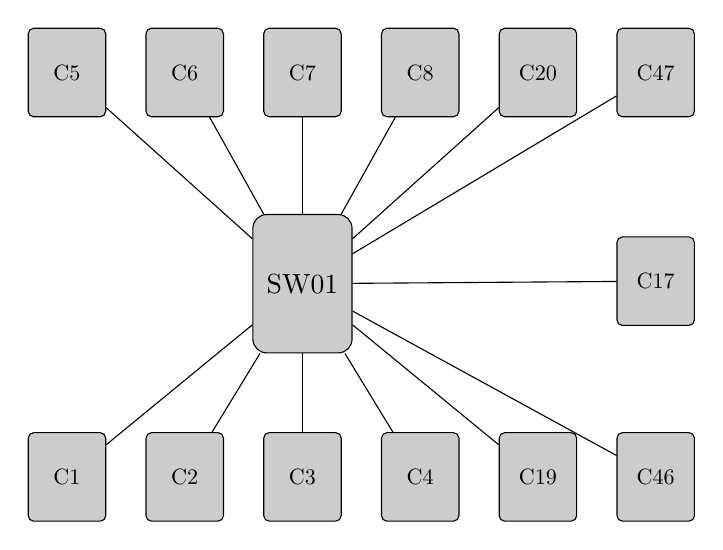
\begin{tikzpicture}[scale=1]

\node[dpu] (C1) at(0,0){C1};

\node[dpu,right=0.5 of C1] (C2) {C2};
\node[dpu,right=0.5 of C2] (C3) {C3};
\node[dpu,right=0.5 of C3] (C4) {C4};
\node[dpu,right=0.5 of C4] (C19) {C19};
\node[dpu,right=0.5 of C19] (C46) {C46};

\node[switch,above=1cm of C3] (SW01) {SW01};

\node[dpu,above=1.35cm of C46] (C17) {C17};
\node[dpu,above=4cm of C1] (C5) {C5};
\node[dpu,right=0.5 of C5] (C6) {C6};
\node[dpu,right=0.5 of C6] (C7) {C7};
\node[dpu,right=0.5 of C7] (C8) {C8};
\node[dpu,right=0.5 of C8] (C20) {C20};
\node[dpu,right=0.5 of C20] (C47) {C47};
\draw (C1) -- (SW01);
\draw (C2) -- (SW01);
\draw (C3) -- (SW01);
\draw (C4) -- (SW01);
\draw (C19) -- (SW01);
\draw (C46) -- (SW01);
\draw (C5) -- (SW01);
\draw (C6) -- (SW01);
\draw (C7) -- (SW01);
\draw (C8) -- (SW01);
\draw (C20) -- (SW01);
\draw (C47) -- (SW01);
\draw (C17) -- (SW01);
%\node[dpu] at (2,0){SCS2};
%\node[dpu] at (2,0){FSSS};
%\node[dpu] at (2,0){吹灰};
%\node[switch] at(2,4){SW01};
%\draw (0,0) rectangle (1,1.5);
%\draw (0.2,0.1) rectangle (1.2,1.6);
\end{tikzpicture}

	\end{frame}
\subsection{各控制器内设备分布}
\begin{frame}{我厂DCS系统架构实例}{控制器内设备分布}
\begin{block}{\heiti 1号锅炉DCS系统各控制器内设备分布}
			\begin{enumerate}
				\item  C1:MCS系统及锅炉涉及的所有PID自动
				
				\item   C2:A侧引风机、送风机、一次风机、空预器,A、C制粉系统相关设备
				
				\item  C3:B侧引风机、送风机、一次风机、空预器,B、D制粉系统相关设备,脱硝系统相关设备
				
				\item  C4:火检冷却风机,密封风机,燃油系统,FSSS系统,汽水系统,锅炉主保护
				
				\pause
				\item  C19:除尘及输灰系统
				\item  C46:本体吹灰
				
		\end{enumerate}
		\end{block}
\end{frame}
\begin{frame}{我厂DCS系统架构实例}{控制器内设备分布}
\begin{block}{\heiti 2、3、4号锅炉设备分布与1号锅炉一致}
			\begin{enumerate}
		
				\item  2号锅炉对应为C5、C6、C7、C8、C20、C47
\pause
				\item  3号锅炉对应为C9、C10、C11、C12、C21、C48
				\pause
				\item  4号锅炉对应为C13、C14、C15、C16、C22、C49
\end{enumerate}
		\end{block}
\begin{alertblock}{\heiti 两台锅炉共用设备!}
			C17为1、2号锅炉除渣系统\\  C18为3、4号锅炉除渣系统
		\end{alertblock}
\end{frame}
\begin{frame}{我厂DCS系统架构实例}{控制器内设备分布}
\begin{block}{\heiti 3号网段各控制器内设备分布}
			\begin{enumerate}
				\item  C29:1号汽轮机:真空泵、凝泵、空冷风机
				
				\item   C30:2号汽轮机:真空泵、凝泵、空冷风机
				
				\item  C36:3号汽轮机	:热力系统阀门
		\end{enumerate}
		\end{block}
\pause
\begin{block}{\heiti 4号网段各控制器内设备分布}
			\begin{enumerate}
				\item  C31:4号汽轮机:油系统、真空泵、凝泵、空冷风机
				
				\item   C32:5号汽轮机:油系统、真空泵、凝泵、空冷风机
		\end{enumerate}
		\end{block}
\pause
\begin{alertblock}{\heiti 每台汽轮机只有一组控制器!}
			凝泵、真空泵、空冷风机、控制油泵、润滑油泵
		\end{alertblock}
\end{frame}
\begin{frame}{我厂DCS系统架构实例}{控制器内设备分布}
\begin{block}{\heiti 5号网段各控制器内设备分布}
			\begin{enumerate}
				

				\item  C33:蒸汽管网:各等级蒸汽系统、除氧器系统、高加系统	

				\item  C34:1号、2号电动给水泵和公用系统	

				\item  C35:3号、4号电动给水泵、汽动给水泵和公用系统	

\item  C23:灰库、C24:煤灰水、 C25:点火油库、C26:压缩空气、C27:化水
			
		\end{enumerate}
		\end{block}
		\begin{alertblock}{\heiti 存在问题:调节阀控制集中在C33控制器}
\begin{itemize}
			\item 所有压力等级管网双减调门\\
			\item 3组高加系统液位调节阀\\
			\item 4组除氧器压力、液位调节阀
\end{itemize}
\end{alertblock}
\end{frame}
\begin{frame}{我厂DCS系统架构实例}{控制器内设备分布}
\begin{block}{\heiti 脱硫DCS系统各控制器内设备分布}
			\begin{enumerate}
				\item  C40:1号脱硫,1号脱硫液氨调门、CEMS数据
				
				\item   C41:2号脱硫,2号脱硫液氨调门、CEMS数据
				
				\item  C42:3号脱硫,3号脱硫液氨调门、CEMS数据

				\item  C43:4号脱硫,4号脱硫液氨调门、CEMS数据

				\item  C44:脱硫公用系统	

				\item  C45:脱硫超低改造增容设备	

		\end{enumerate}
		\end{block}
\pause
\begin{alertblock}{\heiti 单节点系统!}
			AS、CS功能合并为同一台服务器!\\应急措施:液氨调门切至旁路、CEMS数据到站房观察
		\end{alertblock}
\end{frame}
\subsection{重要辅机系统在控制器内分布情况}
\begin{frame}{我厂DCS系统架构实例}{重要辅机系统在控制器内分布情况}
\begin{block}{\heiti 分散布置的系统}
			\begin{enumerate}

				\item  六大风机、空预器、制粉系统分为两组分别分布在两组控制器
				
				\item   4台电动给水泵系统分为两组分别分布在两组控制器
		\end{enumerate}
		\end{block}
\pause
\begin{alertblock}{\heiti 存在问题}
			\begin{enumerate}
				\item  设备分散不彻底,锅炉侧调门、变频器在同一台控制器
				
				\item  主设备停运后触发MFT信号集中在同一台控制器
		\end{enumerate}
		\end{alertblock}
\end{frame}

\begin{frame}{我厂DCS系统架构实例}{重要辅机系统在控制器内分布情况}
\begin{exampleblock}{\heiti 分布在一台控制器}
			\begin{enumerate}
				\item  六大风机入口调门和变频器、4台制粉系统冷热风调门和给煤机变频器、主/辅给水调门
				
				\item  3组高加系统、4组除氧器系统
				
				\item   1、2、3号汽轮机凝结水泵、空冷风机

				\item   4、5号汽轮机控制油泵、润滑油泵、凝结水泵、空冷风机
		\end{enumerate}
		\end{exampleblock}
\pause
\begin{alertblock}{\heiti 风险}
			\begin{enumerate}
				\item  一组控制器故障会影响所有设备!
\item  如果必须执行初始化下装,所有设备会恢复初始状态!
		\end{enumerate}
		\end{alertblock}
\end{frame}
\subsection{重要测点在I/O模件内分布情况}

\begin{frame}{我厂DCS系统架构实例}{重要测点在I/O模件内分布情况}
\begin{alertblock}{\heiti 保护测点分布在同一块卡件}
			\begin{enumerate}
				\item  炉膛压力高高、炉膛压力低低测点
			
		\end{enumerate}
		\end{alertblock}
\pause
\begin{alertblock}{\heiti 调门或变频器指令分布在同一块卡件}
			\begin{enumerate}
				\item  管网双减调节阀指令
				\item  除氧器压力、液位、高压加热器液位调节阀指令
				\item 六大风机入口调门、磨煤机冷热风调门、给煤机指令
			
		\end{enumerate}
		\end{alertblock}
\begin{alertblock}{\heiti DO通道配置有长电平指令设备}
			\begin{enumerate}
				\item  六大风机、空预器、制粉系统停运触发MFT信号
			
		\end{enumerate}
		\end{alertblock}
\end{frame}
\begin{frame}

\begin{table}
	\caption{800XA故障试验结果}
	\begin{tabular}{|c|c|c|c|c|}
		\hline
		       操作    & AI         & DI     & AO&DO  \\   \hline
		卡件故障    & 保持        & 保持      & 保持&保持  \\  \hline 
		更换卡件    & 保持    & 保持   & 复位&复位\\  \hline  
		通讯电缆故障    & 保持        & 保持      & 保持& 保持 \\   \hline  
		站头故障    &保持          & 保持       & 保持& 保持 \\     \hline
CI854故障    &保持          & 保持       & 保持& 保持 \\     \hline
控制器故障    &保持          & 保持       & 保持& 保持 \\     \hline
初始化下装    &复位          & 复位       & 复位& 复位 \\     \hline
	\end{tabular}
	\end{table}
注:站头CI840同时拔出后下属卡件值都会复位


\end{frame}
%\section{DCS典型案例}
\begin{frame}{DCS典型案例}{C3控制器故障处理导致1号锅炉停运}
\begin{block}{\heiti 控制器初始化下装导致锅炉灭火}
			CEX电缆松动导致两台控制器故障且控制器内程序丢失,需要初始化下装逻辑后才能正常运行,将相关设备切至就地后进行初始化下装,下装过程中3台风机变频器跳闸触发炉膛压力低低保护。
		\end{block}
\pause
\begin{alertblock}{\heiti DO电平指令初始化下装过程中复位为0}
			
				检查为风机变频器有软急停电平指令接至DCS DO通道,指令变为0时变频器急停。
			
		
		\end{alertblock}
\end{frame}
\begin{frame}{DCS典型案例}{净化装置控制器故障处理导致全厂停运}
\begin{block}{\heiti 控制器初始化下装导致停车}
			两台控制器故障且控制器内程序丢失,需要初始化下装逻辑后才能正常运行,下装过程调门关闭导致停车
		\end{block}
\pause
\begin{alertblock}{\heiti AO指令初始化下装过程中复位为0}
			
				调节阀指令恢复为0导致调节阀关闭,系统停车
			
		
		\end{alertblock}
\end{frame}
\begin{frame}{DCS典型案例}{所有上位机失电导致工况无法监控调整30分钟}
\begin{block}{\heiti 所有上位机失电导致工况无法监控调整}
			因电气误停UPS电源导致DCS系统公用总电源失电后,所有上位机失电,操作员站、工程师站、各服务器失电导致工况无法监控调整,陆续恢复电源并恢复服务器和操作员站后工况稳定无影响。
		\end{block}
\pause
\begin{alertblock}{\heiti 怎么做???风险!!!
}
			
				紧急停运,停运措施是否完整,风险?\\继续运行,工况是否平稳,风险?
			
		
		\end{alertblock}
\end{frame}

\section{存在的问题与做什么}
\begin{frame}{存在的问题与做什么}{存在的问题}
\begin{alertblock}{\heiti 目前存在问题!!!}
			\begin{enumerate}
				\item  CEX电缆松动会导致一组控制器内程序清空
\item  重要调门集中在同一组控制器上
\item  重要调门AO指令在同一块卡件上未分散
				\item  重要辅机对应控制器故障后具体的处理细节
\item  服务器、工作站备份恢复无法实现
				
				\item  800XA系统各状态有效的监视手段

				\item  网络变量、全局变量的合理使用

				
\item  AO卡件故障后现场对应启动调门应该采取什么措施
		\end{enumerate}
		\end{alertblock}
\end{frame}
\begin{frame}{存在的问题与做什么}{做什么}
\begin{alertblock}{\heiti 下一步做什么???}
			\begin{enumerate}
				\item  合理布置AO调门指令分布
				\item   对现场设备AO、DO指令情况进行具体排查分类确认故障及处理过程中应对措施
\item   DCS系统指令复位时各专业如何保证现场设备保持原状态
				\item   实现备份、恢复服务器
				\item   利用现有备件搭建一套单节点系统


		\end{enumerate}
		\end{alertblock}
\end{frame}


	
	

	
\begin{frame}{排查内容}{排查清单}  
 \begin{thebibliography}{99}

\bibitem{AO} AO指令: \emph{ABB系统AO点排查},
热控专业, 2023-11-16
\bibitem{DO} DO指令: \emph{ABB系统DO点排查},
热控专业, 2023-11-16
\bibitem{AO} 气动调门: \emph{AO供电调节阀},
热控专业, 2023-11-16
\bibitem{AO} 变频器: \emph{变频器远方就地切换状态},
电气专业, 2023-11-16
\end{thebibliography}
\end{frame}
\end{document}
